\section{Theorie}
\label{sec:Theorie}

Geometrische Optik bezeichnet ein Teilgebiet der Physik, in welchem die Ausbreitung des Lichtes durch Strahlen beschrieben wird. Diese werden beim Übergang zwischen zwei Medien mit verschiedenen Brechungsindizes nach dem Brechungsgesetz gebrochen. In der geometrischen Optik werden Linsen verwendet. Es wird zwischen Sammellinsen und Zerstreuungslinsen unterschieden. Eine Sammellinse bündelt einfallende parallel zur optischen Achse verlaufende Lichtstrahlen in einem Punkt, dem Brennpunkt in der Brennweite $f$. Bei der Zerstreuungslinse werden die parallelen Lichtstrahlen gestreut, sodass die Verlängerungen der gestreuten Strahlen sich vor der Linse in einem Punkt kreuzten. Die Brennweite ist somit negativ. Ist die Linse sehr dünn, sodass die Brechung annähernd in einer Mittelebene stattfindet, wird von einer dünnen Linse ansonsten von einer dicken Linse gesprochen. Eine dicke Linse kann angenähert werden, indem die Mittelebene durch zwei Hauptebenen ersetzt wird, an welchen die Strahlen gebrochen werden. Um das Bild eines Gegenstandes zu konstruieren werden meistens drei Strahlen betrachtet. Der Parallelstrahl $P$ verläuft vom Gegenstand aus parallel zur optischen Achse und wird anschließend an der Linse entsprechend gebrochen. Der Mittelpunktstrahl $M$ geht durch die Mitte der Linse, ohne dass sich die Richtung des Strahles außerhalb der Linse ändert. Der Brennpunktstrahl $B$ geht durch den Brennpunkt vor der Linse und wird an der Linse gebrochen, sodass er anschließend parallel zur optischen Achse verläuft. Dort, wo sich die (verlängerten) Strahlen schneiden wird der Punkt, von welchem die drei Strahlen am Gegenstand ausgingen scharf abgebildet. Alle Punkte zusammen ergeben ein Bild, welches reelles Bild genannt wird, falls die Strahlen zur Konstruktion nicht verlängert werden müssen ansonsten virtuelles Bild. Die Konstruktion des Bildes ist in den Abbildungen \ref{1}, \ref{2} und \ref{3} für eine dünne Sammellinse, eine dünne Zerstreuungslinse und eine dicke Sammellinse dargestellt. Das Verhältnis der Bildgröße $B$ zur Gegenstandsgröße $G$ heißt Abbildungsmaßstab $V$ und es folgt aus den Konstruktionsregeln
\begin{equation}
 V = \frac{B}{G}=\frac{b}{g},\label{mast}
\end{equation}
wobei $b$ der Abstand des Bildes und $g$ der Abstand des Gegenstandes zur nächsten Mittelebene bzw. Hauptebene ist. Für dünne Linsen folgt auch die Linsengleichung
\begin{equation}
	\frac{1}{f}=\frac{1}{b}+\frac{1}{g}\label{linsen}
\end{equation}
\begin{figure}
	\centering
	\caption{Die schematische Darstellung der Strahlenverläufe bei einer dünnen Sammellinse \cite{V408}.}
	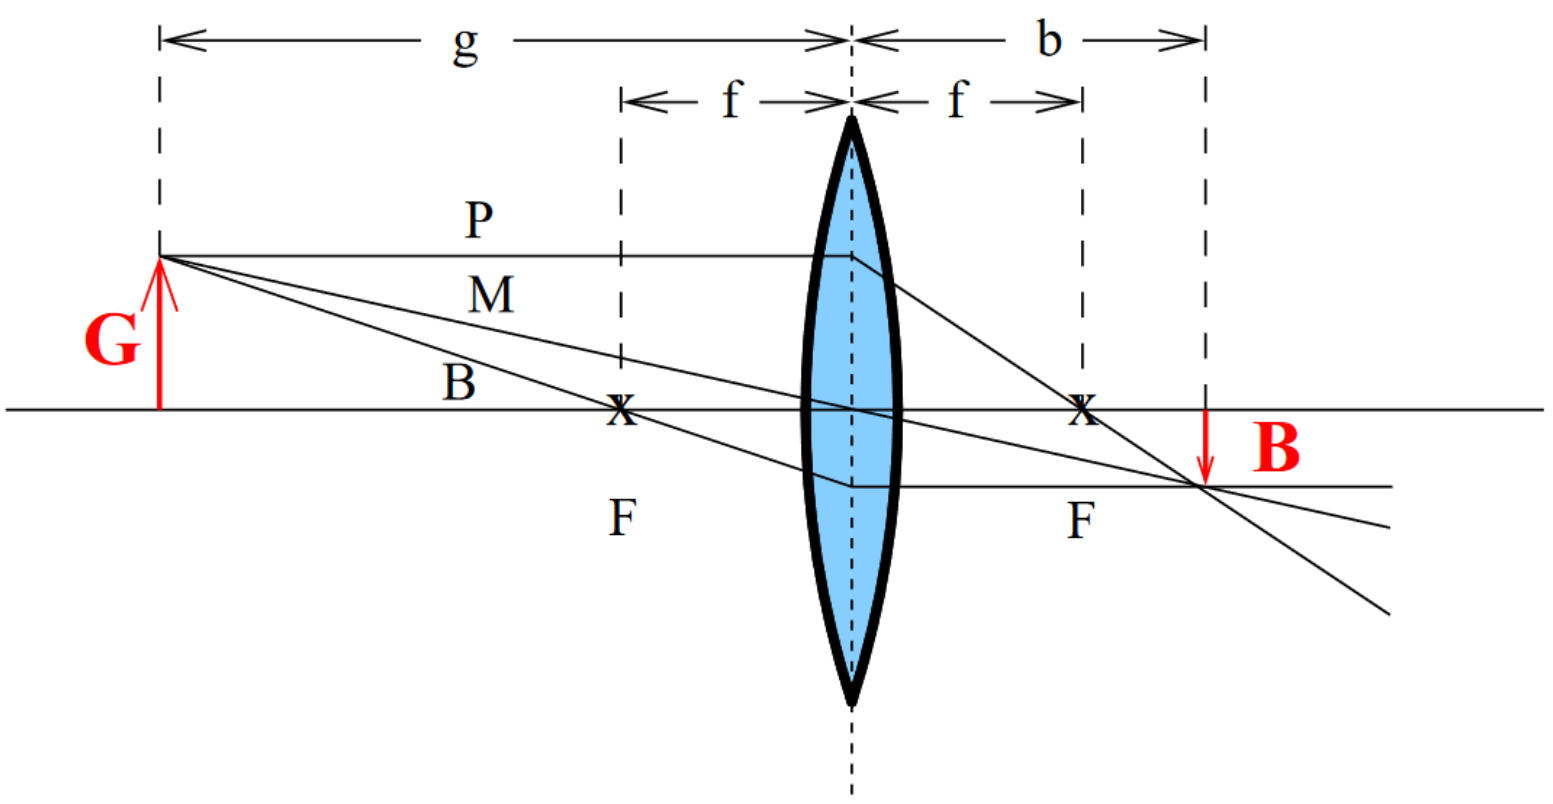
\includegraphics[width=\linewidth-150pt,height=\textheight-150pt,keepaspectratio]{content/images/1.png}
	\label{1}
\end{figure}
\begin{figure}
	\centering
	\caption{Die schematische Darstellung der Strahlenverläufe bei einer dünnen Zerstreuungslinse \cite{V408}.}
	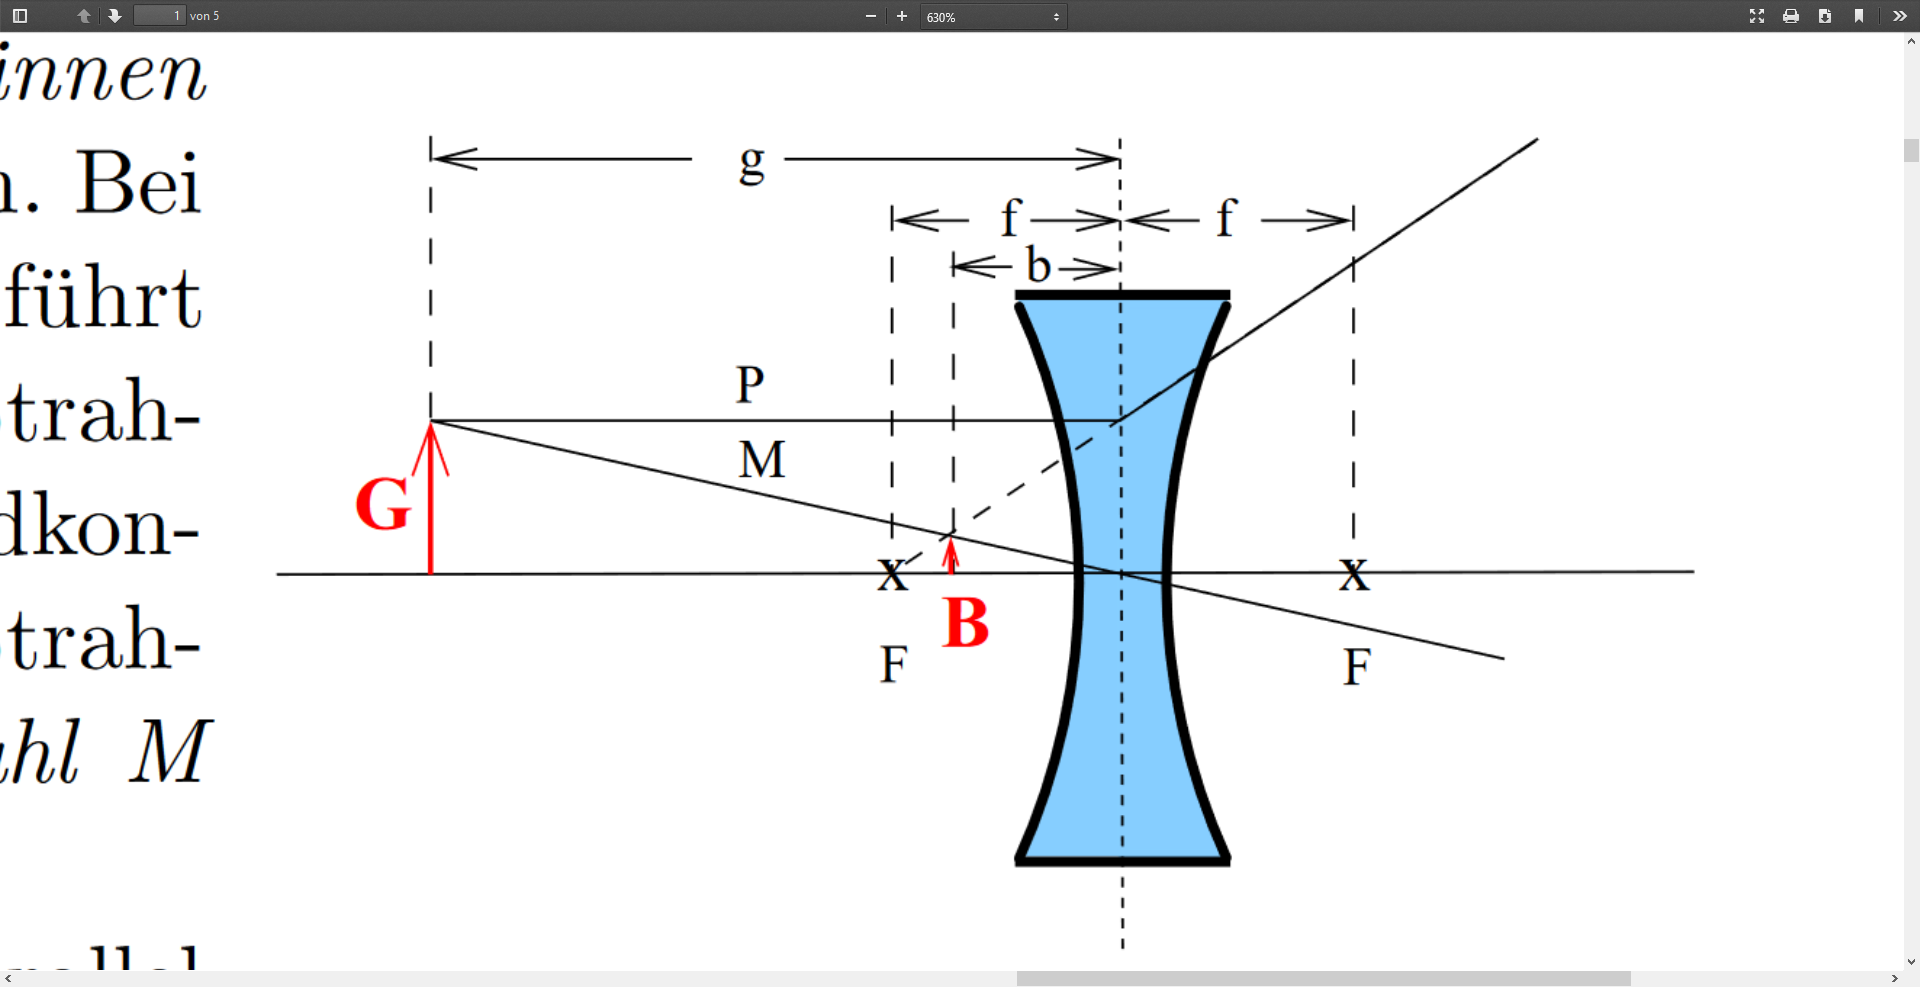
\includegraphics[width=\linewidth-150pt,height=\textheight-150pt,keepaspectratio]{content/images/2.png}
	\label{2}
\end{figure}
\begin{figure}
	\centering
	\caption{Die schematische Darstellung der Strahlenverläufe bei einer dicken Sammellinse \cite{V408}.}
	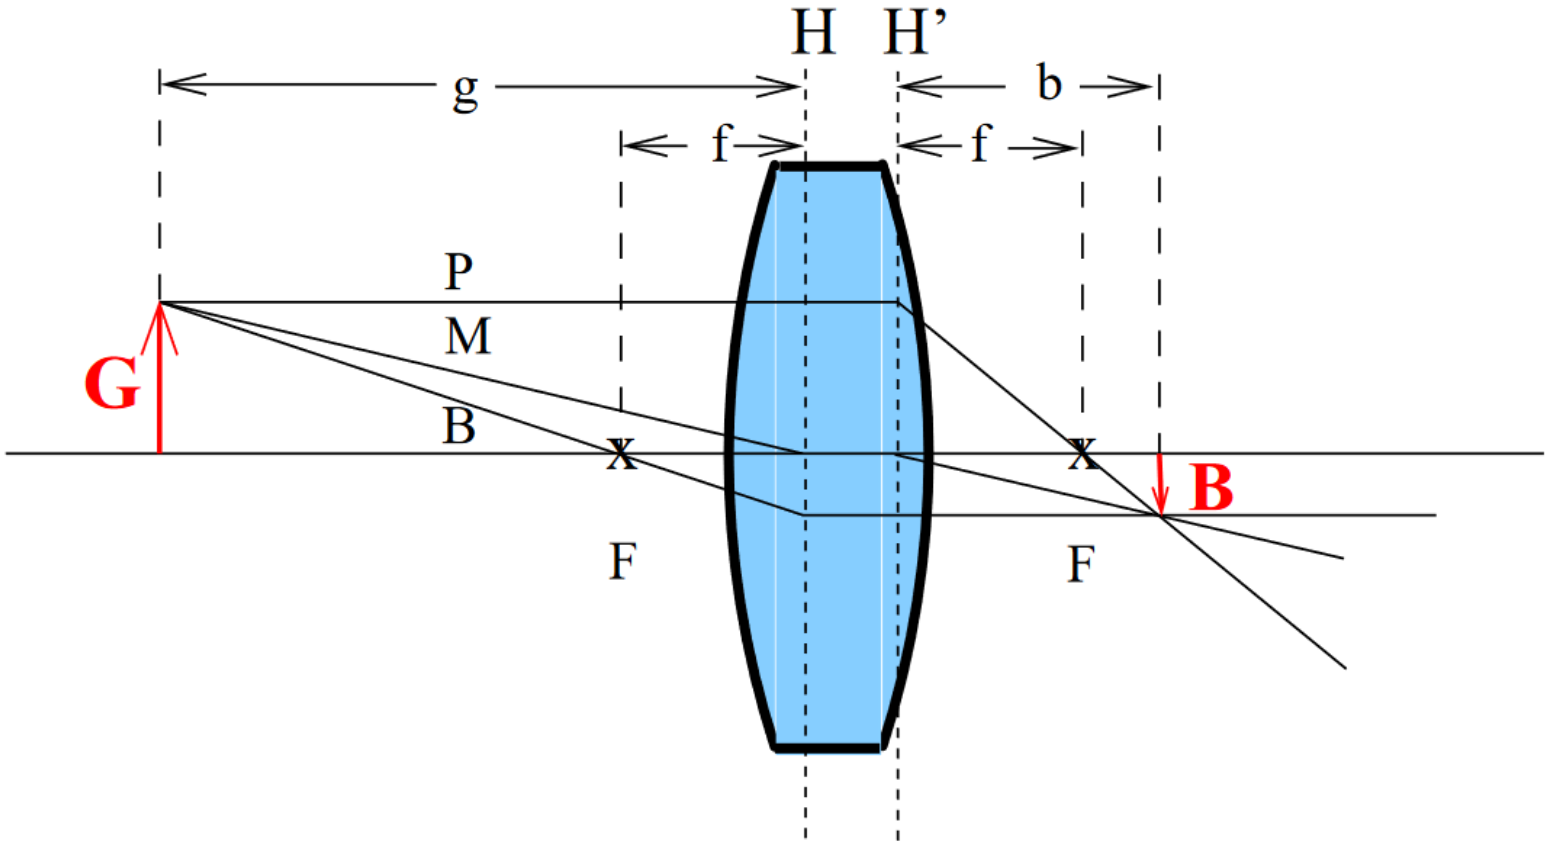
\includegraphics[width=\linewidth-150pt,height=\textheight-150pt,keepaspectratio]{content/images/3.png}
	\label{3}
\end{figure}
Nun gibt es allerdings Effekte, welche die tatsächlichen Verläufe von den theoretischen abweichen lassen. So gilt stellt die Brechung ein der Mittelebene bzw. Hauptebene eine Näherung für achsennahe Strahlen dar. Bei der sphärischen Abberration werden die achsennahen Strahlen weniger stark gebrochen als die achsenfernen, sodass die Brennweite für achsenferne Strahlen geringer ist als für achsennahe. Zudem tritt bei Licht mit unterschiedlichen Wellenlängen auch chromatische Abberation auf, wenn das Licht mit unterschiedlichen Wellenlängen verschieden stark gebrochen wird und somit sich die Brennweite Abhängig von der Wellenlänge des Lichtes ändert. Diese Effekte führen dazu, dass sich das Bild nicht vollkommen scharf stellen lässt.

Um die Brennweite einer Linse experimentell zu bestimmen gibt es mehrere Möglichkeiten. Eine ist die Methode nach Bessel. Hierbei wird der Abstand zwischen Gegenstand und Bild konstant gehalten und die zwei Positionen der Linse gesucht. Durch Einsetzen von der Beziehungen $e=g_1+b_1=g_2+b_2$ und $d=g_1−b_1=g_2−b_2$ in die Linsengleichung \eqref{linsen} ergibt sich
\begin{equation}
	f=\frac{e^2-d^2}{4 e}. \label{unnoetig1}
\end{equation}
Um die Brennweite eines Linsensystems oder einer dicken Linse und die Lage deren Hauptebenen zu bestimmen, kann die Methode von Abbe verwendet werden. Hierbei wird Referenzpunkt $A$ gewählt, welcher sich immer im selben Abstand zum Linsensystem befindet. Zu diesem wird der Abstand vom Gegenstand $g'$ und vom Bild $b'$ gemessen. Aus der Linsengleichung \eqref{linsen} und dem Abbildungsmaßstab $V$ folgt mit den Abständen $h$ bzw. $h'$ der Hauptebenen zu dem Referenzpunkt
\begin{equation}
	g'=g+h=f \cdot \left(1+\frac{1}{V}\right)+h\label{unnoetig2}
\end{equation}
und
\begin{equation}
b'=b+h'=f \cdot \left(1+V\right)+h' .\label{unnoetig3}
\end{equation}
Da $f$, $h$ und $h'$ konstant sind kann z.B durch eine Ausgleichsrechnung die Steigung der Geraden bezüglich $1+1/V$ bzw. $1+V$ bestimmt werden, welche der gesuchten Brennweite entspricht. Der Achsenabschnitt entspricht dann $h$ bzw. $h'$.
Für die theoretische Brennweite zweier Linsen im Abstand von $d$ gilt:
\begin{equation}
  \frac{1}{f_\text{theo}} = \frac{1}{f_1} + \frac{1}{f_2} - \frac{d}{f_1 f_2}\label{theo}
\end{equation}

\begin{figure}
	\centering
	\caption{Die exemplarische Darstellung eines Linsensystems das mit der Methode nach Abbe vermessen werden soll mit eingezeichneten relevanten Größen \cite{V408}.}
	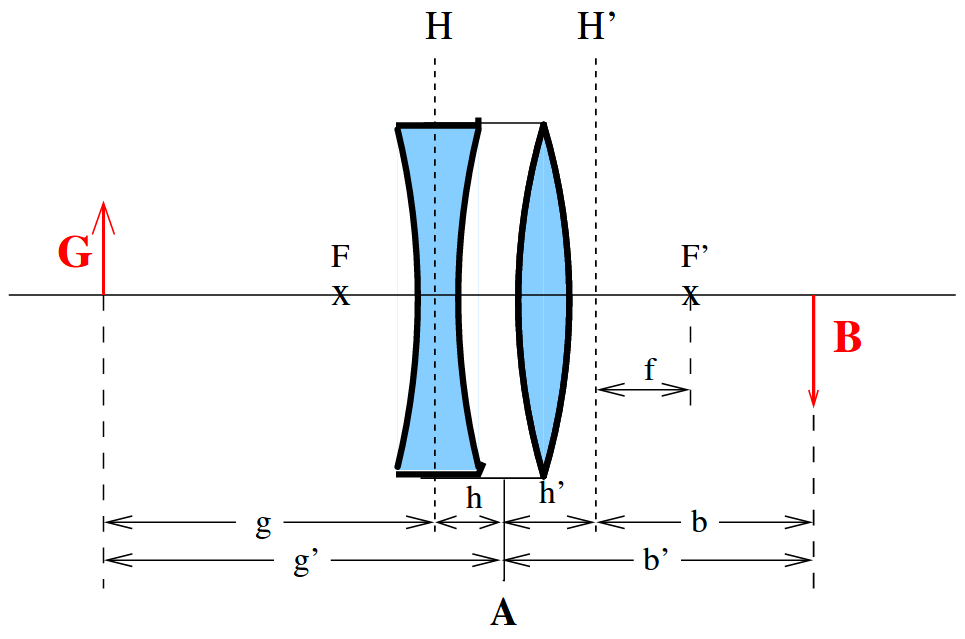
\includegraphics[width=\linewidth-150pt,height=\textheight-150pt,keepaspectratio]{content/images/7.png}
	\label{7}
\end{figure}
